\subsection{Java}
\subsubsection{Java là gì}
\begin{center}
  \captionsetup{type=figure}
  \includesvg[width=4cm]{img/java.svg}
  \captionof{figure}{Java}
\end{center}

Java là một ngôn ngữ lập trình hướng đối tượng (OOP) và dựa trên các lớp (class). Khác với phần lớn ngôn ngữ lập trình thông thường, thay vì biên dịch mã nguồn thành mã máy hoặc thông dịch mã nguồn khi chạy, Java được thiết kế để biên dịch mã nguồn thành bytecode, bytecode sau đó sẽ được môi trường thực thi (runtime environment) chạy.

Trước đây, Java chạy chậm hơn những ngôn ngữ dịch thẳng ra mã máy như C và C++, nhưng sau này nhờ công nghệ "biên dịch tại chỗ" - Just in time compilation, khoảng cách này đã được thu hẹp, và trong một số trường hợp đặc biệt Java có thể chạy nhanh hơn. Java chạy nhanh hơn những ngôn ngữ thông dịch như Python, Perl, PHP gấp nhiều lần. Java chạy tương đương so với C\#, một ngôn ngữ khá tương đồng về mặt cú pháp và quá trình dịch/chạy.

Cú pháp Java được vay mượn nhiều từ C và C++ nhưng có cú pháp hướng đối tượng đơn giản hơn và ít tính năng xử lý cấp thấp hơn. Do đó việc viết một chương trình bằng Java dễ hơn, đơn giản hơn, đỡ tốn công sửa lỗi hơn. Nhưng về lập trình hướng đối tượng thì Java phức tạp hơn.

Trong Java, hiện tượng rò rỉ bộ nhớ hầu như không xảy ra do bộ nhớ được quản lý bởi Java Virtual Machine (JVM) bằng cách tự động "dọn dẹp rác". Người lập trình không phải quan tâm đến việc cấp phát và xóa bộ nhớ như C, C++. Tuy nhiên khi sử dụng những tài nguyên mạng, file IO, database (nằm ngoài kiểm soát của JVM) mà người lập trình không đóng (close) các streams thì rò rỉ dữ liệu vẫn có thể xảy ra.

\subsubsection{Đặc điểm của java}

Java có những đặc điểm cơ bản như sau:
\begin{itemize}
    \item \textbf{Hướng đối tượng:} Trong Java, mọi thứ đều là Object. Java có thể mở rộng vì nó dựa trên mô hình Object.
    \item \textbf{Nền tảng độc lập:} Không giống như nhiều ngôn ngữ lập trình khác (C, C++), khi Java được biên dịch, nó không biên dịch sang một máy tính cụ thể trên nền tảng nào, thay vào đó là những byte code độc lập với nền tảng. Byte code này được phân phối trên web và được thông dịch bằng Virtual Machine (JVM) trên bất cứ nền tảng nào mà nó đang chạy.
    \item \textbf{Đơn giản:} Java được thiết kế để dễ học. Nếu bạn hiểu cơ bản về khái niệm lập trình hướng đối tượng Java, thì có thể nắm bắt ngôn ngữ này rất nhanh.
    \item \textbf{Bảo mật:} Với tính năng an toàn của Java, nó cho phép phát triển những hệ thống không có virus, giả mạo. Các kỹ thuật xác thực dựa trên mã hóa công khai.
    \item \textbf{Kiến trúc trung lập:} Trình biên dịch của Java tạo ra một định dạng file object có kiến trúc trung lập, làm cho code sau khi biên dịch có thể chạy trên nhiều bộ vi xử lý, với sự hiện diện của Java runtime system.
    \item \textbf{Portable:} Là kiến trúc trung lập và không phụ thuộc vào việc thực hiện là những đặc điểm chính nhất khi nói về khía cạnh Portable của Java. Trình biên dịch trong Java được viết bằng ANSI C với một ranh giới portable gọn gàng, đó là một subset POSIX (giao diện hệ điều hành linh động). Bạn có thể mang byte code của Java lên bất cứ nền tảng nào.
    \item \textbf{Mạnh mẽ:} Java nỗ lực loại trừ những tình huống dễ bị lỗi bằng cách nhấn mạnh chủ yếu là kiểm tra lỗi thời gian biên dịch và kiểm tra runtime.
    \item \textbf{Đa luồng:} Với tính năng đa luồng của Java, bạn có thể viết các chương trình có thể thực hiện nhiều tác vụ đồng thời. Tính năng này cho phép các nhà phát triển xây dựng các ứng dụng tương tác có thể chạy trơn tru.
    \item \textbf{Thông dịch:} Byte code của Java được dịch trực tiếp tới các nền tảng gốc và nó không được lưu trữ ở bất cứ đâu. 
    \item \textbf{Hiệu suất cao:} Với việc sử dụng trình biên dịch Just-In-Time, Java cho phép thực thi với hiệu suất cao, nhanh chóng phát hiện, gỡ lỗi.
    \item \textbf{Phân tán:} Java được thiết kế cho môi trường phân tán của Internet.
    \item \textbf{Linh động:} Java được coi là năng động hơn C hay C++ vì nó được thiết kế để thích nghi với môi trường đang phát triển. Các chương trình Java có thể mang theo một lượng lớn thông tin run-time, được sử dụng để xác minh và giải quyết các truy cập đến đối tượng trong thời gian chạy.
\end{itemize}
\subsubsection{Java được dùng ở đâu?}

Ta có thể bắt gặp Java ở rất nhiều nơi, từ những trang web thương mại điện tử đến ứng dụng Android, từ ứng dụng khoa học đến ứng dụng tài chính như hệ thống giao dịch điện tử, trò chơi như Minecrafr đến các ứng dụng trên máy tính như Eclipse, Netbeans, IntelliJ,...
\begin{itemize}
    \item \textbf{Ứng dụng Android:} Nếu muốn nhìn thấy một sản phẩm được tạo ra từ Java thì thật đơn giản, hãy mở điện thoại Android lên và bất kỳ ứng dụng nào bạn nhìn thấy cũng chính là một sản phẩm như vậy, được viết bằng ngôn ngữ lập trình Java, với Android API của Google, tương tự như JDK. Với sự phát triển của Android ngày nay, hầu hết lập trình viên Java đều là những người viết app cho Android. Android sử dụng JVM và cách đóng gói khác nhau, nhưng code thì vẫn được viết bằng Java.
    \item \textbf{Các ứng dụng máy chủ dùng trong dịch vụ tài chính:} Trong ngành dịch vụ tài chính Java chiếm một vị trí khá lớn. Nhiều ngân hàng đầu tư toàn cầu như Goldman Sachs, Citigroup, Barclays, Standard Charted và các ngân hàng khác sử dụng Java để viết hệ thống giao dịch điện tử front office và back office, viết hệ thống giải quyết và xác nhận, dự án xử lý dữ liệu,... Java chủ yếu được sử dụng để viết ứng dụng cho máy chủ, không có front end, nhận dữ liệu từ một máy chủ khác, xử lý nó và gửi đến một tiến trình tiếp theo.
    \item \textbf{Ứng dụng Web:} Java cũng chiếm được một thị phần khá lớn trong lĩnh vực thương mại điện tử và ứng dụng web. Có rất nhiều dịch vụ RESTfull được tạo bằng cách sử dụng Spring MVC, Struts 2.0 và những framework tương tự. Thậm chí những ứng dụng web đơn giản như Servlet, JSP và Struts cũng rất phổ biến trong các dự án khác nhau của chính phủ. Nhiều cơ quan chính phủ, y tế, bảo hiểm, giáo dục, quốc phòng và những bộ phận khác có ứng dụng web được xây dựng bằng Java.
    \item \textbf{Công cụ phần mềm:} Nhiều phần mềm hữu ích và công cụ phát triển được viết và triển khai trong Java, ví dụ như Eclipse, InetelliJ Idea và Netbans IDE. Rất nhiều phần mềm trên máy tính để bàn cũng được viết bằng Java. 
    \item \textbf{Công nghệ Big Data:} Hadoop và các công nghệ dữ liệu lớn khác cũng đang sử dụng Java theo cách này hay cách khác. Apache của Java dựa trên HBase và Accumulo (mã nguồn mở), ElasticSearch cũng vậy. Tuy Java không phải kẻ thống trị trong lĩnh vực này, vì có những công nghệ như MongoDB được viết bằng C ++, nhưng Java có tiềm năng để đạt được thị phần ngày càng tăng nếu Hadoop hoặc ElasticSearch lớn mạnh.
    \item \textbf{Ứng dụng khoa học:} Java thường được lựa chọn mặc định cho các ứng dụng khoa học, bao gồm xử lý ngôn ngữ tự nhiên. Lý do chính là vì Java an toàn hơn, portable, duy trì và đi kèm với những công cụ cấp cao tương đương C++ hay những ngôn ngữ lập trình khác.
\end{itemize}

\subsubsection{Thế mạnh của Java}

Cũng như nhiều ngôn ngữ lập trình khác, trình duyệt Java cũng có cho mình khá nhiều ưu điểm. Trong đó cần được kể tới như: hướng đối tượng rộng, có một nền tảng riêng biệt, có thiết kế đơn giản, khả năng bảo mật cao, nhanh và mạnh.
\begin{itemize}
    \item \textbf{Hướng đối tượng rộng:} Hướng đối tượng rộng trong Java chính là tất cả những thứ đều được mở rộng, trong đó thì Java sẽ được dùng dựa trên các mô hình là Object.
    \item \textbf{Java có nền tảng riêng biệt:} Java có nền tảng riêng biệt, người ta nói như vậy là bởi khi nhận được một câu lệnh nào đó, thì Java sẽ tự động thực hiện biên tập câu lệnh đó sang những Bite Code ở dạng độc lập. Trong đó, Bite Code độc lập này sẽ được hỗ trợ bởi các dịch bằng Vitual Machile với bất cứ phần mềm, ứng dụng nào có sử dụng tới nó.
    \item \textbf{Thiết kế mẫu khá đơn giản:} Không giống như nhiều ngôn ngữ lập trình khác, Java có thiết kế mẫu khá là đơn giản bởi thế mà những nhà lập trình viên không cần phải mất quá nhiều thời gian theo học. Muốn học tốt, thành thạo về Java thì mỗi người chỉ mất từ 1 đến 3 năm là đã có thể thành công.
    \item \textbf{Tính bảo mật cao:} Tính bảo mật cao, chính là một ưu điểm của Java so với các trình duyệt khác. Trong đó, khả năng của Java là phát hiện được những thành phần có chứa các virut độc hại, rồi sau đó nó cũng có thể “tiêu diệt” được  virut đó. Để thực hiện được điều này, những nhà lập trình viên ra Java đã phát triển cho nó những thuật toán ở mức độ cao nhất.
    \item \textbf{Nhanh và mạnh:} Đối với ưu điểm này, Java là một trình duyệt có được khả năng xử lý những tình huống bị xảy ra trên máy chủ rất nhanh. Bên cạnh đó, nó cũng có được khả năng truyền dẫn về internet với tốc độ cao, không kém gì những ứng dụng khác.
\end{itemize}

\subsubsection{Framework Spring}
\begin{center}
  \captionsetup{type=figure}
  
\includegraphics[width=15cm]{img/spring.png}
  \captionof{figure}{Spring Java}
\end{center}

Spring là framework phát triển ứng dụng phổ biến nhất dành cho Java Enterprise. Ban đầu nó được viết bởi Rod Johnson và lần đầu tiên được phát hành theo giấy phép Apache 2.0 vào tháng 6 năm 2003. Spring có kích thướng nhẹ, phiên bản cơ bản của Spring framework có kích thước khoảng 2MB.

Spring framework là một Java Platform mã nguồn mở, một giải pháp gọn nhẹ dành cho Java Enterprise. Với Spring Framework các nhà phát triển có thể tạo ra các mã có hiệu suất cao, dễ kiểm thử và có thể sử dụng lại được.

Các tính năng core của Spring Framework có thể được sử dụng trong việc phát triển bất kỳ ứng dụng Java nào. Bên cạnh đó, phần mở rộng được sử dụng để xây dựng các ứng dụng web trên nền tảng Java EE. Mục tiêu của Spring Framework là làm cho việc phát triển ứng dụng J2EE dễ dàng hơn và thúc đẩy việc lập trình tốt hơn bằng mô hình POJO-based.
\begin{center}
  \captionsetup{type=figure}
  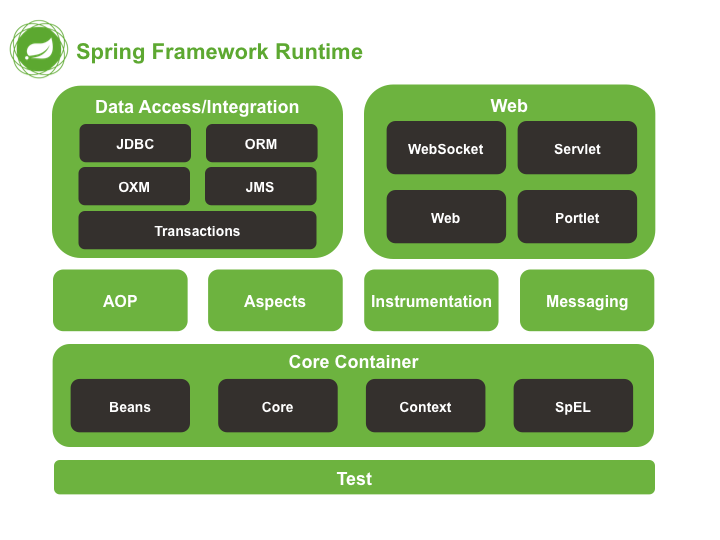
\includegraphics[width=15cm]{img/spring_runtime.png}
  \captionof{figure}{Spring Framework Runtime}
\end{center}

\subsubsection{Điểm mạnh của Framework Spring}

Dưới đây là danh sách các lợi ích tuyệt vời của việc sử dụng Spring Framework:
\begin{itemize}
    \item Spring cho phép các nhà phát triển tạo các ứng dụng cấp Enterprise sử dụng các POJO. Lợi ích của việc sử dụng các POJO là bạn không cần một sản phẩm chứa EJB như một máy chủ ứng dụng, mà bạn chỉ có thể sử dụng một bộ chứa servlet mạnh mẽ như Tomcat hoặc một số sản phẩm thương mại khác.
    \item Spring được tổ chức theo kiểu mô đun. Mặc dù số lượng các gói và các lớp là khá nhiều, nhưng bạn chỉ cần quan tâm đến những gì bạn cần và không cần quan tâm đến phần còn lại.
    \item Spring sử dụng một số công nghệ hiện có như một số ORM Framework, logging frameworks, JEE, Quartz, JDK timers và các công nghệ View khác.
    \item Dễ dàng để kiểm thử một chương trình được viết bằng Spring.
    \item Web framework của Spring là một Web MVC framework có thiết kế tốt, nó là một thay thế tuyệt vời cho Struts và các công nghệ kém phổ biến khác.
    \item Spring cung cấp một API thuận tiện để dịch các ngoại lệ công nghệ cụ thể (ném bởi JDBC, Hibernate, hoặc JDO chẳng hạn) vào các trường hợp ngoại lệ nhất quán, không được kiểm soát.
    \item IoC Container có trọng lượng nhẹ. Điều này có lợi cho việc phát triển và triển khai các ứng dụng trên các máy tính có bộ nhớ và tài nguyên CPU hạn chế.
    \item Spring cung cấp một giao diện quản lý transaction nhất quán có thể mở rộng đến một local transaction (ví dụ như sử dụng một cơ sở dữ liệu) và mở rộng lên các global transaction (sử dụng JTA).
\end{itemize}